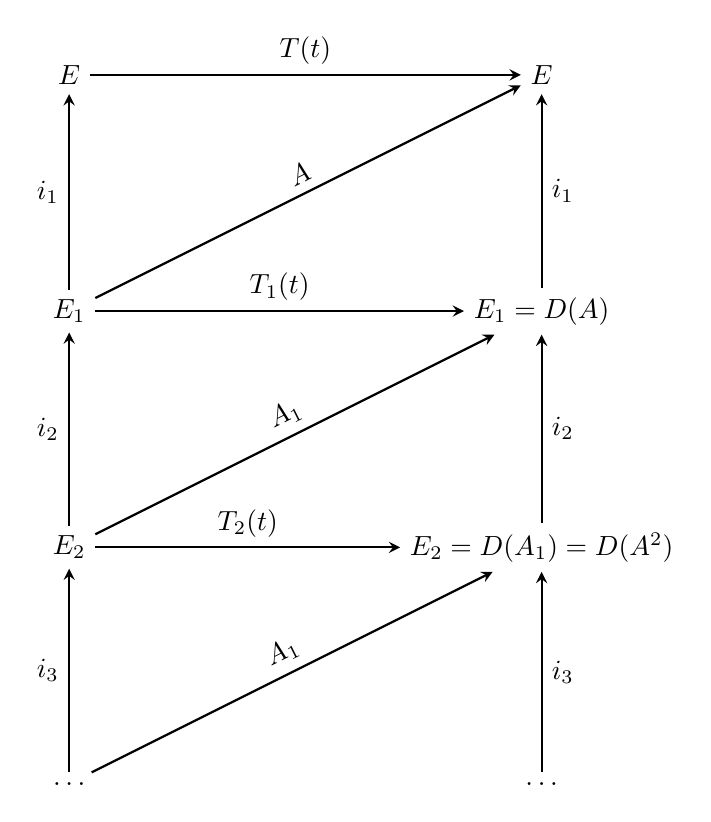
\begin{tikzpicture}[>=stealth]
    % Knoten direkt definieren
    \node (E1) at (0,6) {$E$};
    \node (E2) at (0,3) {$E_1$};
    \node (E3) at (0,0) {$E_2$};
    \node (E4) at (0,-3) {$\ldots$};
    
    \node (F1) at (6,6) {$E$};
    \node (F2) at (6,3) {$E_1 = D(A)$};
    \node (F3) at (6,0) {$E_2 = D(A_1) = D(A^2)$};
    \node (F4) at (6,-3) {$\ldots$};
    
    % Horizontale Pfeile
    \draw[thick,->] (E1) -- node[above] {$T(t)$} (F1);
    \draw[thick,->] (E2) -- node[above] {$T_1(t)$} (F2);
    \draw[thick,->] (E3) -- node[above] {$T_2(t)$} (F3);
    
    % Vertikale Pfeile links
    \draw[thick,->] (E2) -- node[left] {$i_1$} (E1);
    \draw[thick,->] (E3) -- node[left] {$i_2$} (E2);
    \draw[thick,->] (E4) -- node[left] {$i_3$} (E3);
    
    % Vertikale Pfeile rechts
    \draw[thick,->] (F2) -- node[right] {$i_1$} (F1);
    \draw[thick,->] (F3) -- node[right] {$i_2$} (F2);
    \draw[thick,->] (F4) -- node[right] {$i_3$} (F3);
    
    % Diagonale Pfeile
    \draw[thick,->] (E2) -- node[above, sloped] {$A$} (F1);
    \draw[thick,->] (E3) -- node[above, sloped] {$A_1$} (F2);
    \draw[thick,->] (E4) -- node[above, sloped] {$A_1$} (F3);
\end{tikzpicture}